Alternative text, or `Alt text', is a textual description of an equation, link or figure that can be used to replace the visual information in that element. This is often seen as a text `pop-up' in PDF readers. 

Alt text can be added after the PDF is compiled using a PDF editor such as Adobe's Acrobat Pro. 

Alternatively -- and probably best for ensuring that the final document is what the author intended -- the pop up can be generated from within the source document using the \verb+\pdftooltip+ environment from the \emph{pdfcomment} package. For example, \verb?\pdftooltip{a^2+b^2=c^2}{An equation}? produces a pop-up when the cursor passes over the equation:

\begin{equation}
\pdftooltip{a^2+b^2=c^2}{An equation}
\end{equation}

The same approach can be used to create alt text for images. Figure \ref{fig:TestImagesWithAltText} has been labeled with a tool tip. 

\begin{figure*}
	\begin{subfigure}[t]{.45\linewidth}
		\centering
		{\pdftooltip{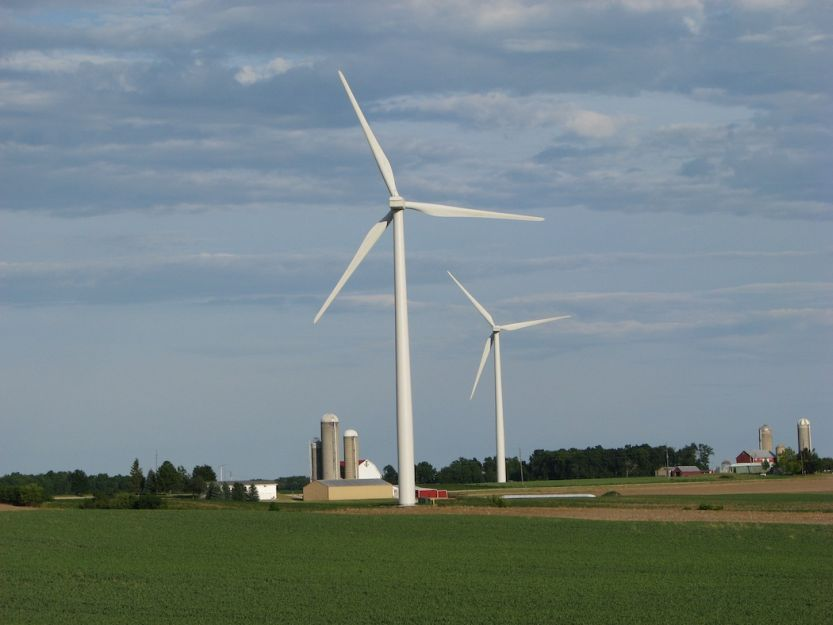
\includegraphics[height=2in]{../DemoFiles/21206.jpg}}{Wind turbines standing in a rural area at the Forward Wind Energy Center in Fond du Lac and Dodge Counties, Wisconsin. (Photo by Ruth Baranowski / NREL)}}
		\caption{Wind turbines at the Forward Wind Energy Center in Fond du Lac and Dodge Counties, Wisconsin. (Photo by Ruth Baranowski / NREL)}\label{fig:21206WithAltText}
	\end{subfigure}%
	\hfill
	\begin{subfigure}[t]{.45\linewidth}
		\centering
		{\pdftooltip{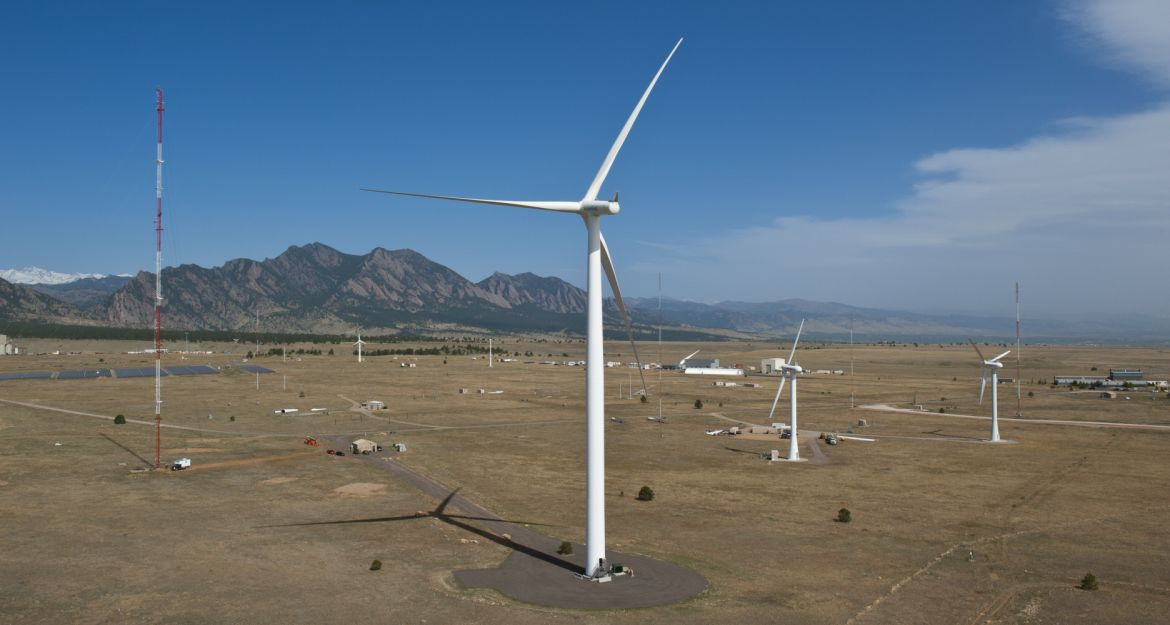
\includegraphics[height=2in]{../DemoFiles/20018.jpg}}{A view from the air of the National Wind Technology Center. (Photo by Dennis Schroeder / NREL)}}
            \caption{Aerial view of the National Wind Technology Center. (Photo by Dennis Schroeder / NREL)}\label{fig:20018WithAltText2}
	\end{subfigure}
	\caption{Testing images with alt-text}\label{fig:TestImagesWithAltText}
\end{figure*}